From last part we know that answer is a line but in this question we must minimize two cost function so there is two line and seven unknowns.

Equations:
$$x_1(t) = c_1t +c_2 \quad 0\leq t \leq t_1$$
$$x_2(t) = c_3t +c_4 \quad t_1 \leq t \leq t_f$$


Boundary condition:



Initial time: 
$\theta_0(t) = t^2 $
$$(g + (\dot{\theta}-\dot{x})g_{\dot{x}}) \vert_{t = t_0}= 0 \to \sqrt{1+\dot{x}^2} + (2t -\dot{x} )\dfrac{\dot{x}}{\sqrt{1+\dot{x}^2}}\vert_{t = t_0} = 0 \to t_0 = -\dfrac{1}{2\dot{x}}\vert_{t = t_0}$$
$$\to t_0 = -\dfrac{1}{2c_1} \to t_0 + \dfrac{1}{2c_1} = 0$$
$$\theta_0(t_0) = x_1(t_0) = t_0^2 = c_1t_0 + c_2 \to t_0^2 - c_1t_0 - c_2 = 0 $$
Final time: 
$\theta_f(t) = t-1 $
$$(g + (\dot{\theta}-\dot{x})g_{\dot{x}})\vert_{t = t_f}  = 0 \to \sqrt{1+\dot{x}^2} + (1-\dot{x}) \dfrac{\dot{x}}{\sqrt{1+\dot{x}^2}}\vert_{t = t_f} = 0 \to \dot{x}_f = -1$$
$$\to c_3 = -1$$
$$\theta_f(t_f) = x_2(t_f) = t_f -1 = -t_f + c_4 \to 2t_f - c_4 -1 = 0 $$
Corner conditions:
$\theta_c(t) = 4 + 2(t-4)^2$
$$(g + (\dot{\theta}-\dot{x})g_{\dot{x}}) \vert_{t = t_1^-} = (g + (\dot{\theta}-\dot{x})g_{\dot{x}}) \vert_{t = t_1^+} $$
$$\to -4t_1 + 16 = 4t_1c_1 -16c_1 \to 4t_1(c_1+1) - 16c_1 -16 = 0$$
In $t = t_1$:
$$\theta_0(t_1) = \theta_f(t_1) \to c_1t_1+c_2 = -t_1 + c_4$$
$$c_1t_1+c_2  +t_1 - c_4 = 0$$
$$\theta_0(t_1) = \theta_c(t_1) = \theta_f(t_1)$$
$$\to c_1t_1 + c_2 = 4 + 2(t_1-4)^2 \to 2(t_1-4)^2 + 4 -c_1t_1 - c_2 = 0$$
The above equations solved if MATLAB (Q3\_d.m).



\begin{table}[H]
	\caption {Answers} \label{ans} 
	\begin{center}
		\begin{tabular}{| l | l | l | l | l | l |}
			\hline
			$t_0$ & $x_0$ & $t_1$ & $x_1$ & $t_f$ & $x_f$ \TBstrut \\
			\hline
			$2.11$ & $4.448$ & $4$ & $4$ & $4.5$ & $3.5$ \Tstrut\\
			\hline
		\end{tabular}
	\end{center}
\end{table}
$x_1(t) = -0.237t+4.9483, \quad x_2(t) = -t + 8$
\begin{figure}[H]
	\caption{Answer function with corner}
	\centering
	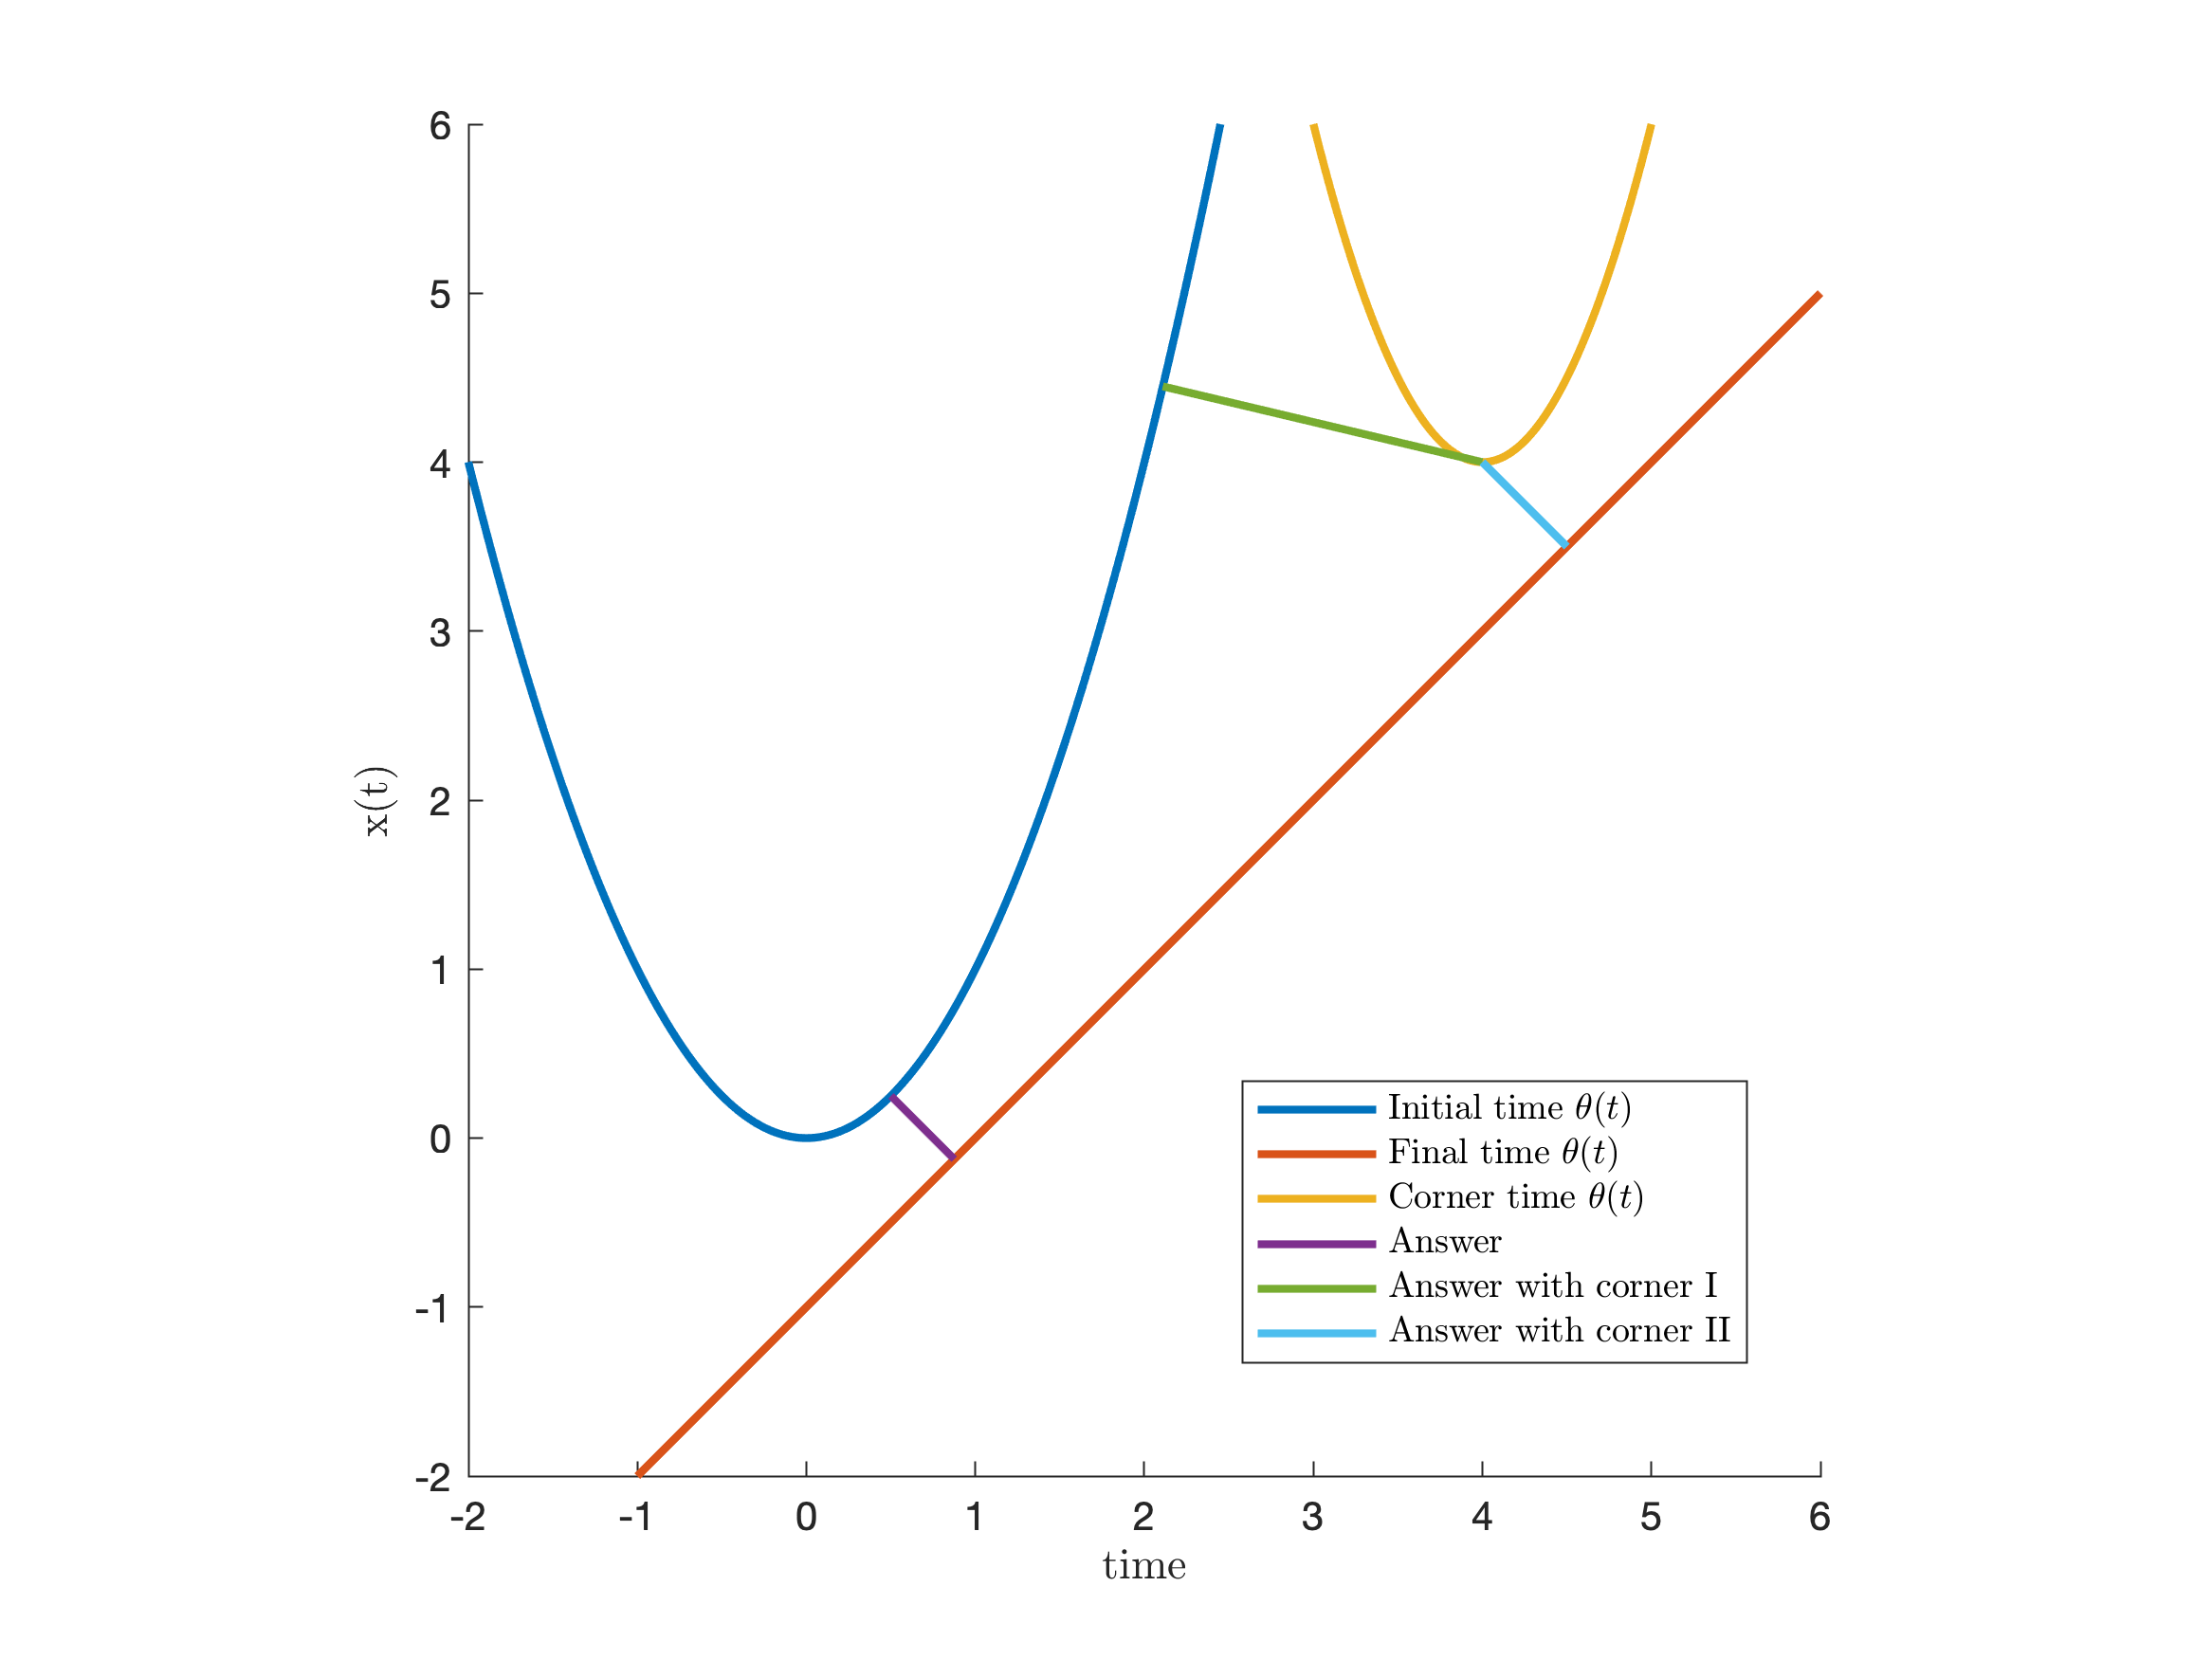
\includegraphics[width=12cm]{Q3/figures/Q3WithCornerFixFigure.png}
\end{figure}
